\documentclass{article}
\usepackage{pgfplots}
\pgfplotsset{width=10cm,compat=1.9}
%\usetikzlibrary{external}
%\tikzexternalize

\begin{document}
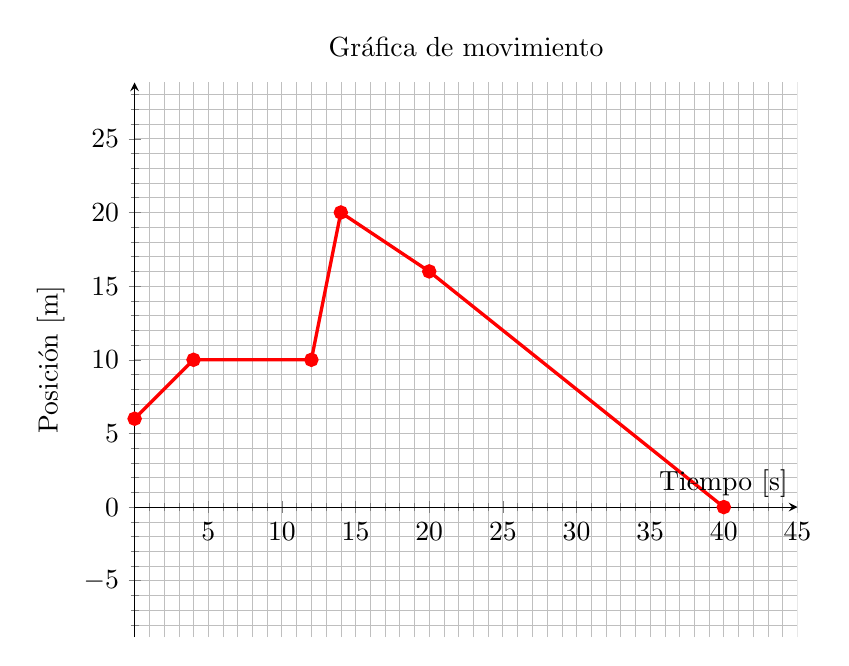
\begin{tikzpicture}
    \begin{axis}[
        title={Gráfica de movimiento},
        xlabel={Tiempo [s]},
        ylabel={Posición [m]},
        xmin=0, xmax=45,
        ymin=-5, ymax=25,
        axis lines=left,
        axis x line=middle,
        axis equal=true,
        %xtick={0,20,40,60,80,100},
        %ytick={0,20,40,60,80,100,120},
        xtick distance=5,
        ytick distance=5,
        minor tick num=4,
        grid=both,
        grid style={solid,lightgray},
        minor grid style={solid,very thin},
        ]

        \addplot[
            color=red,
            style=very thick,
            mark=*,
        ]
        coordinates {
                (0,6)(4,10)(12,10)(14,20)(20,16)(40,0)
            };

        %\node [red,font=\small,anchor=south west] at (axis cs:14,20) {(14,20)};
        %\node [red,font=\small,anchor=south west] at (axis cs:20,16) {(20,16)};

    \end{axis}
\end{tikzpicture}
\end{document}